% Appendix D: road bumps (exploratory). Decided 2026-10-08: in the paper as an exploratory
% appendix only (revising the earlier "not in the paper"). Source: DOCUMENTATION.md 6.8,
% SIMULATION_METHODS.md 3.15 and 4.9; numbers from outputs/scooter_sim/[suspension/]bumps/
% (bump_fall_counts.csv, bump_rear_check_thresholds.csv) and keyframes/keyframes_runs.csv.

\section{Road bumps: an exploratory extension of the model}\label{app:bumps}

\textbf{Status.} These are exploratory model results, not findings about real scooters.
No bump was measured or identified on the rides, and the model's behaviour on bumps has
not been validated. Everything below describes what the simulation produced under its
assumed parameters (Table~\ref{tab:4}) and the analyst-chosen fall criteria
(section~\ref{dynamics-model}).

\textbf{Why bumps.} Raised obstacles, such as a utility cover or patch standing proud of
the surface, a lifted slab, a tree-root ridge or a traffic-calming hump, are a second
kind of road irregularity a rider may meet. Whether they matter for e-scooter riders in
practice is not tested here.

\textbf{What was simulated.} The dynamics model of section~\ref{dynamics-model}, unchanged
except for the road:
\begin{itemize}
\item \emph{Sharp-edged rectangular bumps}, 20--100 mm high, 300, 600 and 1000 mm long (the
  pothole lengths), with MuJoCo's contact. This idealised shape stands for defects: legal
  UK road humps may not have a vertical face above 6 mm \autocite{roadhumps1999}.
\item \emph{Round-top (circular-arc) humps}, 20--100 mm high, 3.7 m long, the round-top
  length reported as standard \autocite{tal2_96}, and 600 mm long (shorter than the 900 mm
  legal minimum, as might be found off the highway), with the profile contact.
\item The same sharp bumps with the profile contact, as a cross-check of the contact model.
\item Speeds of 15, 20 and 25 km/h, configurations 10/10, 12/10, 12/12 and 14/10, without
  and with the modelled front spring; and a rear-size check on the 300 mm sharp bump
  (heights 50--100 mm in 5 mm steps, seven configurations including larger rear wheels).
\end{itemize}
In the fall attribution, a fall is credited to the rear wheel if the rear wheel had
reached the bump's leading face before the fall criterion was met.

\begin{table}[htbp]
\centering\small
\caption{Number of runs meeting the fall criteria, per configuration (sharp bumps and
potholes: of 81 runs; round-top humps: of 54).}\label{tab:D1}
\begin{tabular}{@{}llrrrr@{}}
\toprule
Obstacle & Fork & 10/10 & 12/10 & 12/12 & 14/10 \\
\midrule
Pothole (sharp) & none & 15 & 14 & 14 & 11 \\
Sharp bump & none & 22 & 13 & 14 & 4 \\
Round-top hump & none & 0 & 0 & 0 & 0 \\
\addlinespace
Pothole (sharp) & front spring & 9 & 6 & 6 & 1 \\
Sharp bump & front spring & 1 & 2 & 1 & 2 \\
Round-top hump & front spring & 0 & 0 & 0 & 0 \\
\bottomrule
\end{tabular}
\end{table}

\begin{table}[htbp]
\centering\small
\caption{Rear-size check, 300 mm sharp bump: lowest bump height (mm, 5 mm steps) at which
the model met the fall criteria; -- = not met up to 100 mm.}\label{tab:D2}
\begin{tabular}{@{}llrrrrrrr@{}}
\toprule
Fork & Speed & 10/10 & 12/10 & 14/10 & 10/12 & 12/12 & 10/14 & 14/14 \\
\midrule
none & 15 km/h & 85 & 95 & -- & 85 & 95 & 85 & -- \\
none & 20 km/h & 80 & 90 & 100 & 80 & 90 & 80 & 100 \\
none & 25 km/h & 80 & 85 & 100 & 80 & 85 & 80 & 95 \\
\addlinespace
front spring & 15 km/h & 85 & 85 & 85 & 90 & 95 & -- & 100 \\
front spring & 20, 25 km/h & -- & -- & -- & -- & -- & -- & -- \\
\bottomrule
\end{tabular}
\end{table}

\textbf{Observations (model only).}
\begin{enumerate}
\item \emph{Without the front spring}, the current configuration met the fall criteria in
  more sharp-bump runs than pothole runs of the same dimensions (22 against 15 of 81;
  Table~\ref{tab:D1}). A plausible geometric explanation, not tested separately, is that a
  wheel meets the full height of a step but drops only part way into a short pothole.
  Fewer falls occurred with larger front wheels (22, 13 and 4 for 10, 12 and 14 in fronts);
  changing the rear size alone did not change the falling heights (Table~\ref{tab:D2}).
  Figure~\ref{fig:D1} shows one case.
\item \emph{With the front spring}, bump falls were rare: one or two runs per configuration,
  all on the 300 mm bump at 15 km/h. In each, the fall criteria were met after the rear
  wheel struck the bump's leading edge (Figure~\ref{fig:D2}). In the rear-size check, a
  larger rear wheel raised the falling height or prevented the fall (10/12: 90 mm; 12/12:
  95 mm; 14/14: 100 mm; 10/14: none up to 100 mm), while a larger front wheel alone did
  not (85 mm for 10/10, 12/10 and 14/10). This rests on very few runs (one bump length, one
  speed, differences of 5--15 mm, close to the 5 mm step) and on a model not validated
  for bumps. It is reported as an open question, whether rear-wheel size or rear
  suspension matters on scooters with a sprung front, not as evidence that larger rear
  wheels are more stable. It does indicate that the working hypothesis of this paper (the
  front wheel alone) may not hold for every type of obstacle.
\item No round-top hump run met the fall criteria in any configuration, consistent with,
  but not evidence for, guidance that humps can be ridden safely by cyclists and
  motorcyclists \autocite{tal7_96}; that guidance was not written for e-scooters. The
  short 600 mm hump gave large modelled speed losses at 15 km/h (up to 47\% with the
  fork).
\item The front spring changed the bump results much more than the pothole results (10/10:
  22 to 1 falls on bumps, 15 to 9 on potholes), so the bump results depend strongly on
  the assumed fork stiffness, damping and travel, which were not varied for bumps.
\end{enumerate}

\begin{figure}[htbp]
\centering
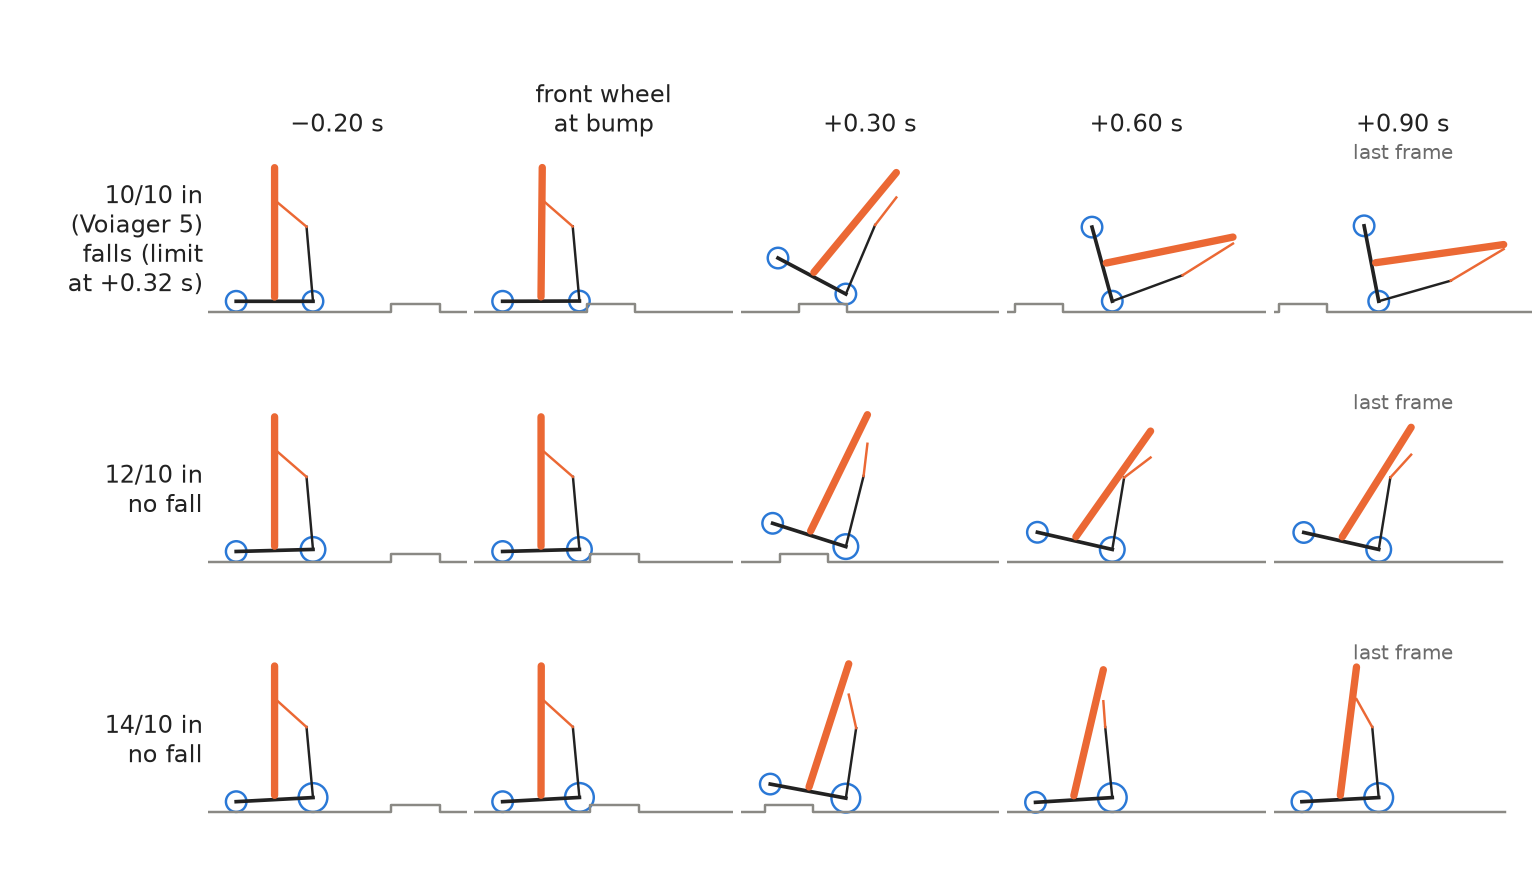
\includegraphics[width=\linewidth]{fig_d1_bump_keyframes.png}
\caption{Key frames, sharp-edged bump 90 mm high and 600 mm long at 20 km/h, model
without front suspension. Columns: the same moments in each row, relative to the front
wheel reaching the bump. The current configuration pitches forward after the front-wheel
strike; with 12 in and 14 in front wheels the model rolls over the bump. Drawn as in
Figure~\ref{fig:5}.}\label{fig:D1}
\end{figure}

\begin{figure}[htbp]
\centering
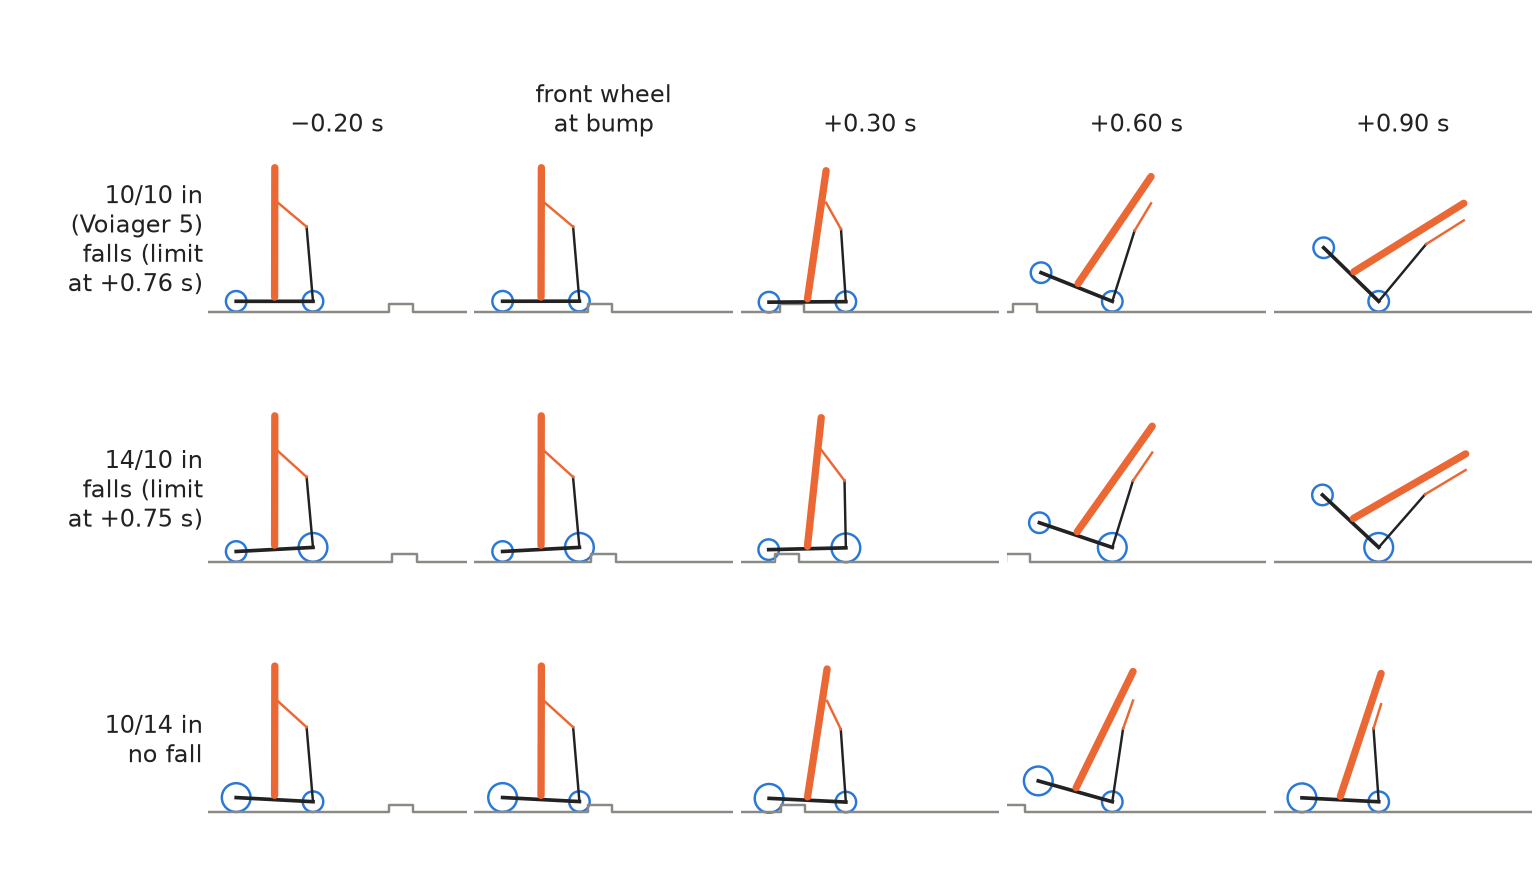
\includegraphics[width=\linewidth]{fig_d2_bump_rear_strike.png}
\caption{Key frames, short sharp-edged bump 90 mm high and 300 mm long at 15 km/h, model
with the front spring. The front wheels cross; about 0.3 s later the rigid rear wheel
strikes the edge and, with 10 in rear wheels, the scooter pitches forward. With a 14 in
rear wheel (10/14) the model does not fall. One run per configuration; an open question,
not a result about rear-wheel size (text).}\label{fig:D2}
\end{figure}

Figures~\ref{fig:Dfallsa}--\ref{fig:Dgb} give the full bump results behind Table~\ref{tab:D1}.

\FloatBarrier

\begin{figure}[htbp]
\centering
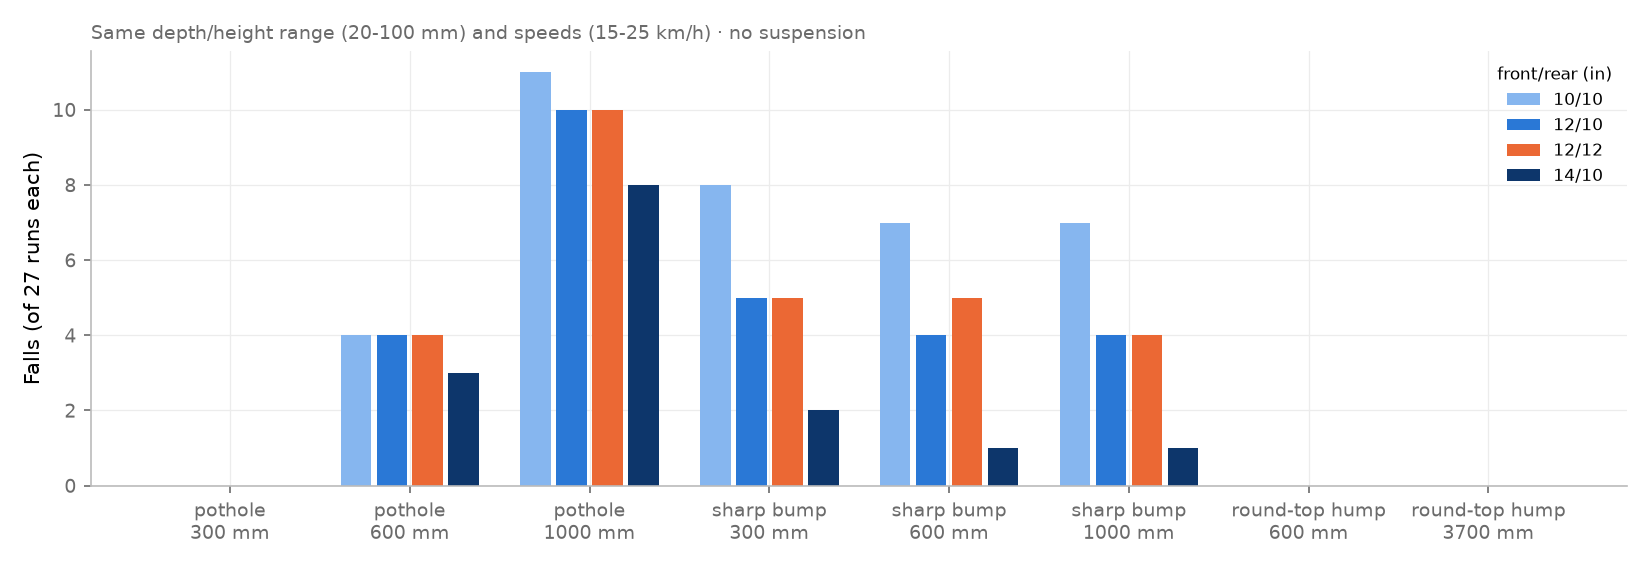
\includegraphics[width=\linewidth]{sim/bump_falls_nofork.png}
\caption{Falls by obstacle type and length, model without front suspension, per wheel configuration (same depth or height range, 20--100 mm, and speeds, 15--25 km/h). Exploratory; bump results are not validated against measurements.}\label{fig:Dfallsa}
\end{figure}

\begin{figure}[htbp]
\centering
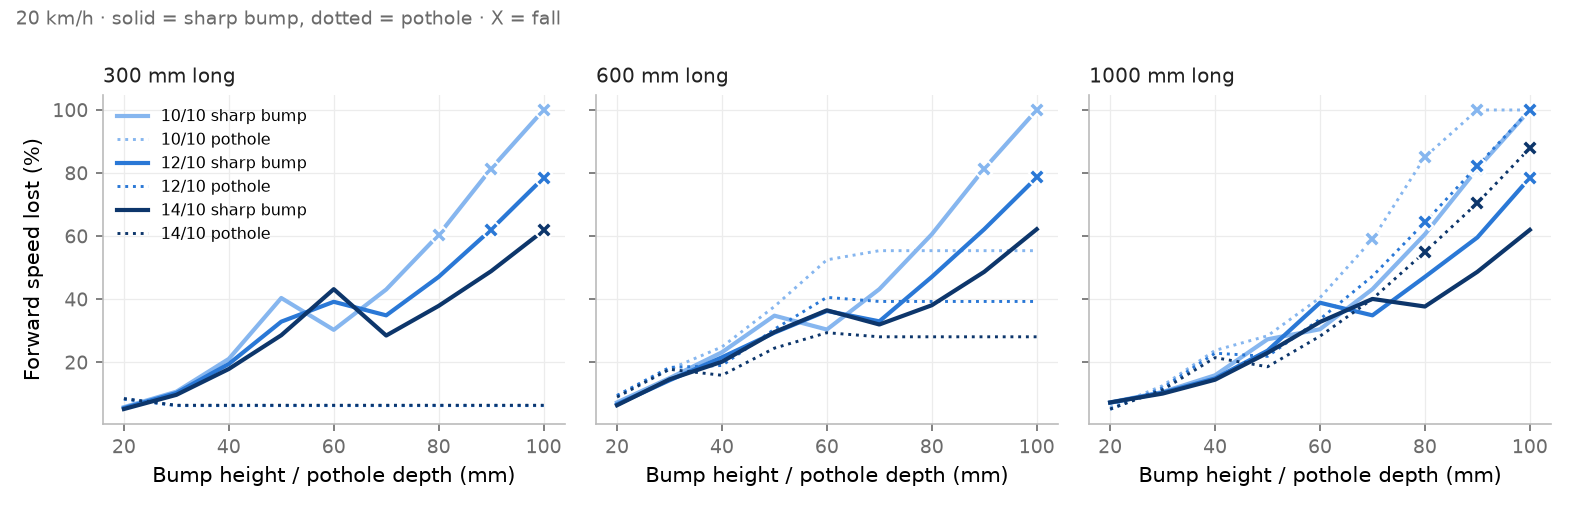
\includegraphics[width=\linewidth]{sim/bump_vs_pothole_nofork.png}
\caption{Forward speed lost on sharp-edged bumps (solid) and potholes of the same size (dotted), 20 km/h, model without front suspension; X marks a fall. Exploratory; bump results are not validated against measurements.}\label{fig:Dvsa}
\end{figure}

\begin{figure}[htbp]
\centering
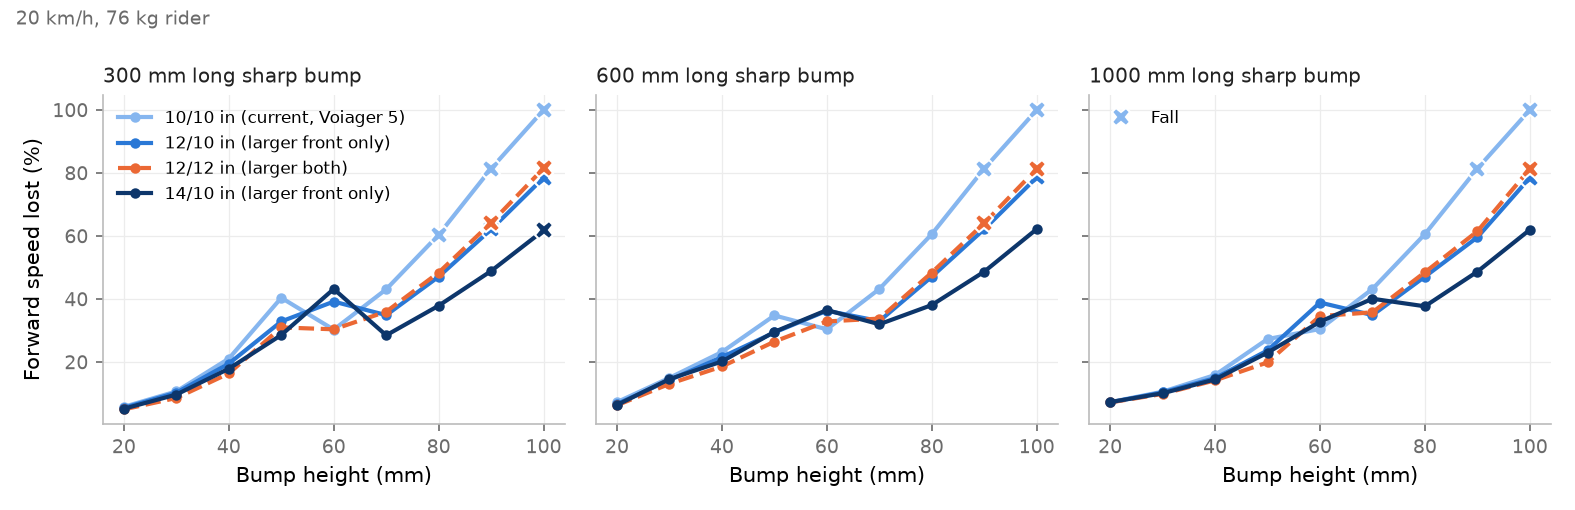
\includegraphics[width=\linewidth]{sim/bump_speedloss_nofork.png}
\caption{Forward speed lost on bumps by height, length and wheel configuration, model without front suspension. Exploratory; bump results are not validated against measurements.}\label{fig:Dspeeda}
\end{figure}

\begin{figure}[htbp]
\centering
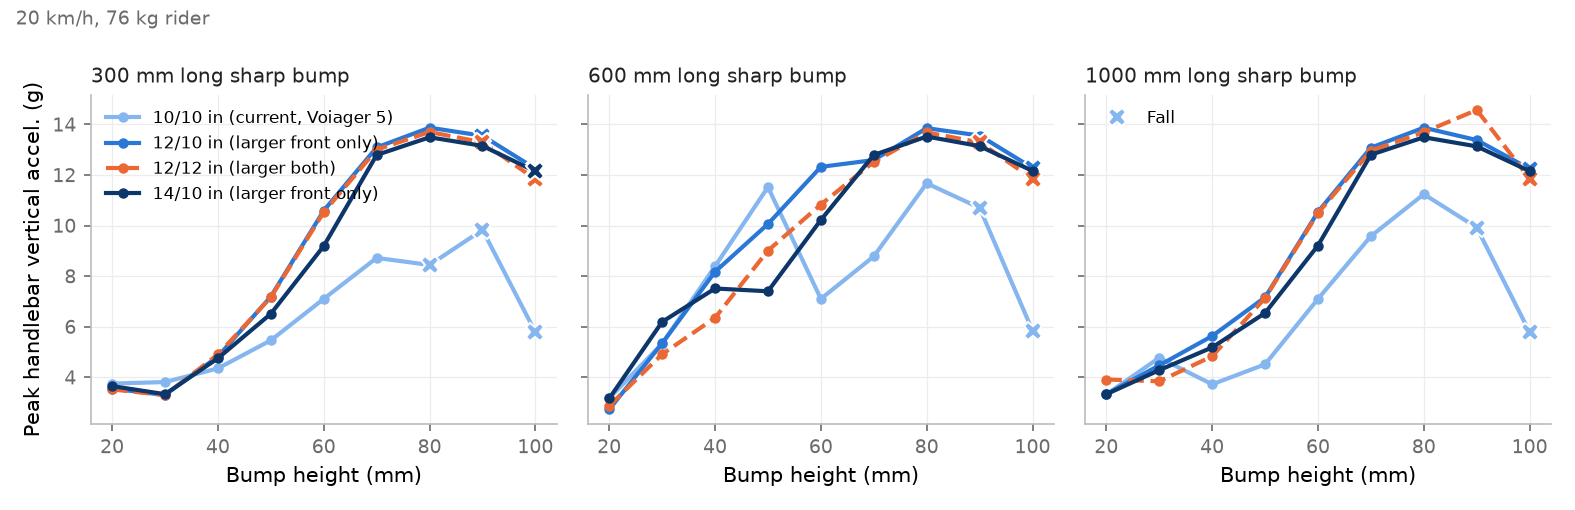
\includegraphics[width=\linewidth]{sim/bump_handlebar_nofork.png}
\caption{Simulated handlebar peak on bumps, model without front suspension. Values above the measured 1.0--2.97 g range are not supported by any measurement. Exploratory; bump results are not validated against measurements.}\label{fig:Dga}
\end{figure}

\begin{figure}[htbp]
\centering
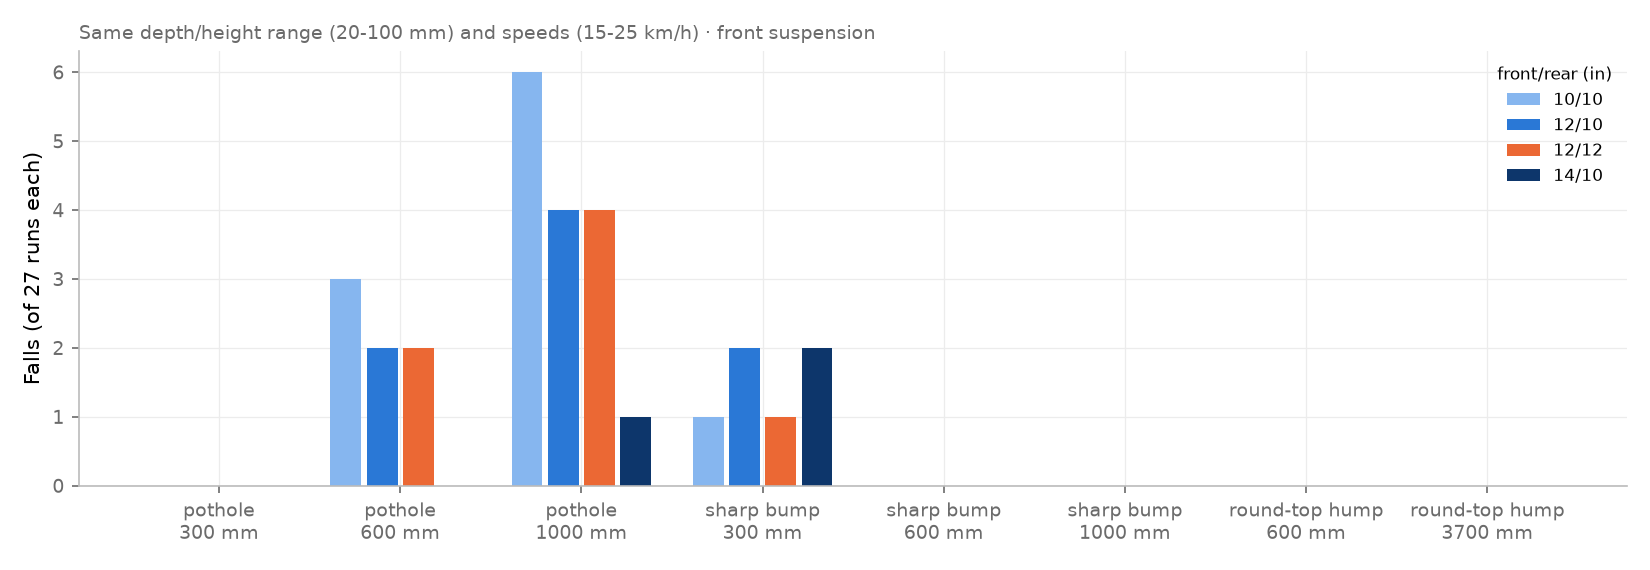
\includegraphics[width=\linewidth]{sim/bump_falls_fork.png}
\caption{Falls by obstacle type and length, model with the front spring, per wheel configuration (same depth or height range, 20--100 mm, and speeds, 15--25 km/h). Exploratory; bump results are not validated against measurements.}\label{fig:Dfallsb}
\end{figure}

\begin{figure}[htbp]
\centering
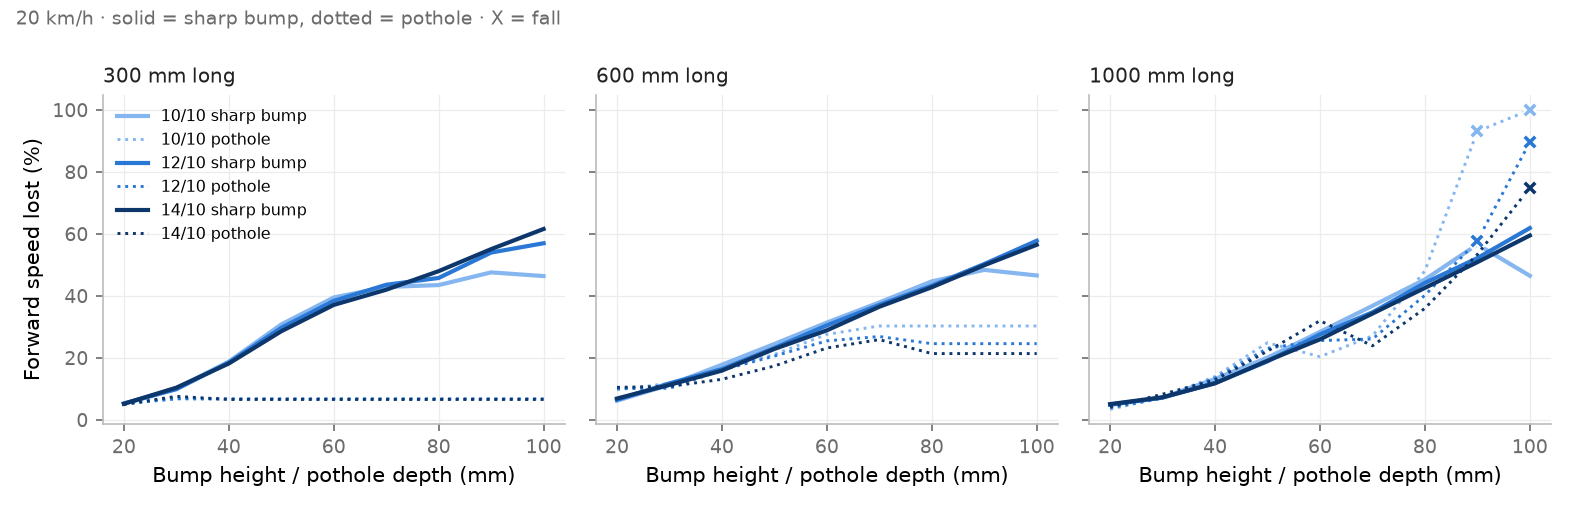
\includegraphics[width=\linewidth]{sim/bump_vs_pothole_fork.png}
\caption{Forward speed lost on sharp-edged bumps (solid) and potholes of the same size (dotted), 20 km/h, model with the front spring; X marks a fall. Exploratory; bump results are not validated against measurements.}\label{fig:Dvsb}
\end{figure}

\begin{figure}[htbp]
\centering
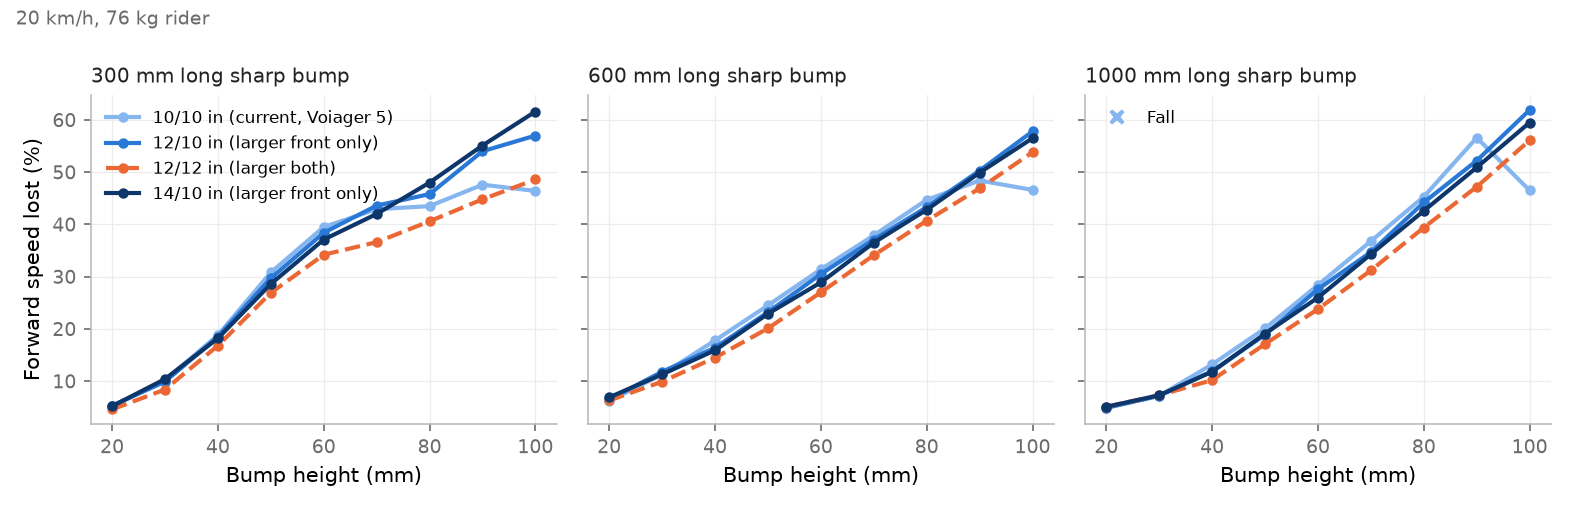
\includegraphics[width=\linewidth]{sim/bump_speedloss_fork.png}
\caption{Forward speed lost on bumps by height, length and wheel configuration, model with the front spring. Exploratory; bump results are not validated against measurements.}\label{fig:Dspeedb}
\end{figure}

\begin{figure}[htbp]
\centering
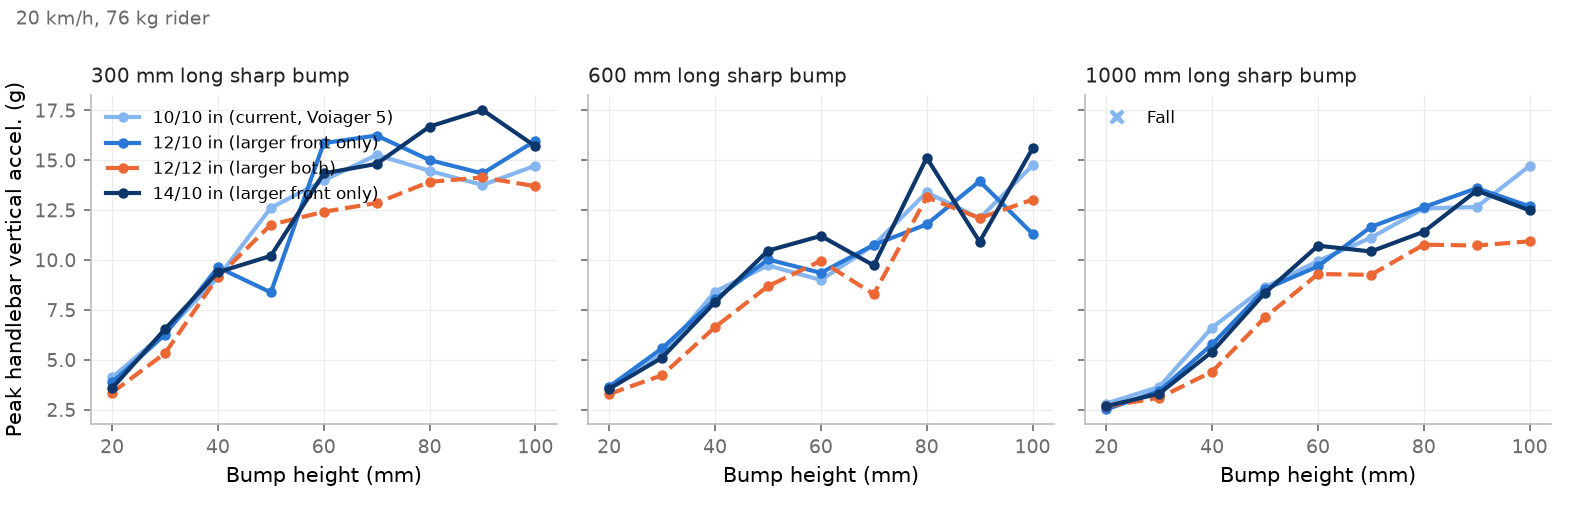
\includegraphics[width=\linewidth]{sim/bump_handlebar_fork.png}
\caption{Simulated handlebar peak on bumps, model with the front spring. Values above the measured 1.0--2.97 g range are not supported by any measurement. Exploratory; bump results are not validated against measurements.}\label{fig:Dgb}
\end{figure}

\textbf{Uncertainties and what these results cannot show.}
\begin{itemize}
\item \emph{Contact model.} On sharp bumps the two contact models agreed on the fall outcome
  in 295 of 324 runs without the fork and 307 of 324 with it (potholes: 30 of 30), with
  disagreements in both directions; the cause is not established.
\item \emph{No validation.} Modelled jolts on sharp bumps (for example 3.6--8.4 g at
  20--40 mm, 600 mm long, 20 km/h, with the fork) exceed the 1.0--2.97 g measured for 99
  of the 100 impacts in Part A, and no bumps were identified on the rides to compare with.
\item \emph{No sensitivity analysis} for bumps (tyre, rider bracing, fork parameters), and
  rear sizes were varied only on the 300 mm bump.
\item \emph{Simplifications} as for potholes: planar model, no steering, coasting, rigid rider
  pinned at the feet, idealised shapes, assumed rear wheel size.
\item \emph{Not shown:} that real bumps cause falls, that bumps are more or less dangerous than
  potholes on the road, any injury risk, or that any wheel size is safe.
\end{itemize}
